\documentclass[10pt]{article}

\usepackage[utf8]{inputenc}
\usepackage[spanish]{babel}
\usepackage{amsmath}
\usepackage[margin=2.5cm]{geometry}
\usepackage{setspace}
\usepackage{graphicx}
\usepackage{tikz}
\usetikzlibrary{circuits.logic.US}

\usepackage{booktabs}   
\usepackage{ragged2e}
\usepackage[table]{xcolor} 
\usepackage{tabularx}  
\usepackage{longtable} 
\usepackage{caption}    
\usepackage{float}
\usepackage{makecell}

\usepackage{booktabs}
\usepackage{listings}

\lstdefinestyle{rstyle}{
  language=R,
  basicstyle=\ttfamily\small,
  keywordstyle=\bfseries,
  commentstyle=\itshape,
  breaklines=true,
  frame=single,
  columns=flexible,
  keepspaces=true,
  showstringspaces=false
}

\usepackage{enumitem}
\newlist{glosario}{description}{1}
\setlist[glosario]{
    font=\normalfont\bfseries,
    leftmargin=0pt,
    labelsep=0.5em,
    itemsep=0.5em
}

\newcommand{\relleno}[1][\textbf{[COMPLETAR AQUÍ]}]{\textcolor{red}{#1}}
\usepackage{colortbl}
\usepackage[colorlinks=true,linkcolor=black,urlcolor=black,citecolor=black]{hyperref}

\definecolor{tablebackground}{rgb}{0.8, 0, 0}
\newcolumntype{x}[1]{>{\centering\arraybackslash\hspace{0pt}}p{#1}}
\newcolumntype{M}[1]{>{\centering\arraybackslash}m{#1}}
\newcolumntype{N}{@{}m{0pt}@{}}
\newcolumntype{P}[1]{>{\RaggedRight\arraybackslash}p{#1}}

\newcommand{\itemEmail}{ccapatinta@unsa.edu.pe}
\newcommand{\itemStudent}{Camilo B.A. Capatinta Almanza}
\newcommand{\itemCourse}{Lab. Estadística matemática, probabilidades y métodos empíricos}
\newcommand{\itemCourseCode}{2502223}
\newcommand{\itemSemester}{IV}
\newcommand{\itemUniversity}{Universidad Nacional de San Agustín de Arequipa}
\newcommand{\itemFaculty}{Facultad de Ingeniería de Producción y Servicios}
\newcommand{\itemDepartment}{Departamento Académico de Ingeniería de Sistemas e Informática}
\newcommand{\itemSchool}{Escuela Profesional de Ingeniería de Sistemas}
\newcommand{\itemAcademic}{2026 - B}
\newcommand{\itemInput}{09/10/2026}
\newcommand{\itemOutput}{16/10/2026}
\newcommand{\itemPracticeNumber}{02}
\newcommand{\itemTheme}{Probabilidad aplicada a la salud pública: tasas de mortalidad y pruebas diagnósticas con R}

\usepackage{fancyhdr}
\pagestyle{fancy}
\fancyhf{}
\setlength{\headheight}{40.51407pt}
\renewcommand{\headrulewidth}{1pt}
\renewcommand{\footrulewidth}{1pt}

\fancyhead[L]{\raisebox{-0.2\height}{
\includegraphics[width=3cm]{img/logo_episunsa.png}}}
\fancyhead[C]{\fontsize{7}{7}\selectfont    \itemUniversity \\ \itemFaculty \\ \itemDepartment \\ \itemSchool \\ \textbf{\itemCourse}}
\fancyhead[R]{\raisebox{-0.2\height}{
\includegraphics[width=1.2cm]{img/logo_abet.png}}}

\fancyfoot[L]{Capatinta Camilo}
\fancyfoot[C]{\itemCourse}
\fancyfoot[R]{Página \thepage}

\begin{document}

	\vspace*{10px}
	
	\begin{center}
		\parbox{0.8\textwidth}{\centering\fontsize{17}{20}\selectfont\textbf{Informe de laboratorio \itemPracticeNumber}}
	\end{center}
	\begin{center}
		\parbox{0.8\textwidth}{\centering\textbf{\Large Tema: \itemTheme}}
	\end{center}

\begin{flushright}
    \begin{tabular}{|M{2.5cm}|N|}
        \hline 
        \rowcolor{tablebackground}
        \color{white} \textbf{Nota}  \\
        \hline 
             \\[30pt]
        \hline          
    \end{tabular}
\end{flushright}    

\begin{table}[h!]
    \begin{tabular}{|x{4.7cm}|x{4.8cm}|x{4.8cm}|}        
        \hline 
        \rowcolor{tablebackground}
        \color{white} \textbf{Estudiante} & \color{white}\textbf{Escuela}  & \color{white}\textbf{Asignatura}   \\
        \hline 
        {\itemStudent \par \itemEmail} & \itemSchool & {\itemCourse \par Semestre: \itemSemester \par Código: \itemCourseCode}     \\
        \hline          
    \end{tabular}
\end{table}     

\begin{table}[H]
    \begin{tabular}{|x{4.7cm}|x{4.8cm}|x{4.8cm}|}
        \hline 
        \rowcolor{tablebackground}
        \color{white}\textbf{Laboratorio} & \color{white}\textbf{Tema}  & \color{white}\textbf{Duración}   \\
        \hline 
        \itemPracticeNumber & \itemTheme & 02 horas   \\
        \hline 
    \end{tabular}
\end{table}

\begin{table}[H]
    \begin{tabular}{|x{4.7cm}|x{4.8cm}|x{4.8cm}|}
        \hline 
        \rowcolor{tablebackground}
        \color{white}\textbf{Semestre académico} & \color{white}\textbf{Fecha de inicio}  & \color{white}\textbf{Fecha de entrega}   \\
        \hline 
        \itemAcademic & \itemInput &  \itemOutput  \\
        \hline 
    \end{tabular}
\end{table}

\newpage
\tableofcontents
\thispagestyle{plain}
\clearpage

\section{Actividades}
 
\subsection{Ejercicio 4.9: tasas de mortalidad en África Oriental}
 
\subsubsection*{Enunciado}
Se dispone de un subconjunto de las estadísticas vitales de la OMS (datos recolectados entre 1995 y 2000 y reportados en 2003). Los datos incluyen la tasa de mortalidad (\texttt{dr}, por cada 1000 habitantes al año) de los países de África Oriental. Se elige una persona al azar de África Oriental y se pregunta, para cada caso, de qué país o países podría provenir:
\begin{itemize}
  \item Si su probabilidad de morir durante el próximo año es mayor que $0.0167$.
  \item Si su probabilidad de morir durante el próximo año es menor que $0.0067$.
  \item Si su probabilidad de morir durante el próximo año es mayor que $0.00167$ y menor que $0.0181$.
\end{itemize}
 
\subsubsection*{Datos}
La fila \textit{Eastern Africa} (18.8) corresponde al agregado regional y no a un país, por lo que no se considera en el análisis. La probabilidad de morir en un año se obtiene como $p = \mathrm{dr}/1000$.
 
\begin{table}[htbp]
  \centering
  \caption{Tasa de mortalidad (por 1000 al año) y probabilidad asociada.}
  \begin{tabular}{lrr}
    \toprule
    País & dr & $p = \mathrm{dr}/1000$ \\
    \midrule
    Burundi & 20.6 & 0.0206 \\
    Comoros & 8.4 & 0.0084 \\
    Djibouti & 17.7 & 0.0177 \\
    Eritrea & 11.9 & 0.0119 \\
    Ethiopia & 17.7 & 0.0177 \\
    Kenya & 16.7 & 0.0167 \\
    Madagascar & 13.2 & 0.0132 \\
    Malawi & 24.1 & 0.0241 \\
    Mauritius & 6.7 & 0.0067 \\
    Mozambique & 23.5 & 0.0235 \\
    Reunion & 5.5 & 0.0055 \\
    Rwanda & 21.8 & 0.0218 \\
    Somalia & 17.7 & 0.0177 \\
    Uganda & 16.7 & 0.0167 \\
    United Republic of Tanzania & 18.1 & 0.0181 \\
    Zambia & 28.0 & 0.0280 \\
    Zimbabwe & 27.0 & 0.0270 \\
    \bottomrule
  \end{tabular}
\end{table}
 
\subsubsection*{Desarrollo en R}
Una tasa de mortalidad por 1000 es una frecuencia relativa, así que la probabilidad de que una persona de un país muera el próximo año es $p = \mathrm{dr}/1000$. Cada inciso se reduce a filtrar los países cuya $p$ cumple la desigualdad pedida.
 

\begin{figure}[H]
\centering
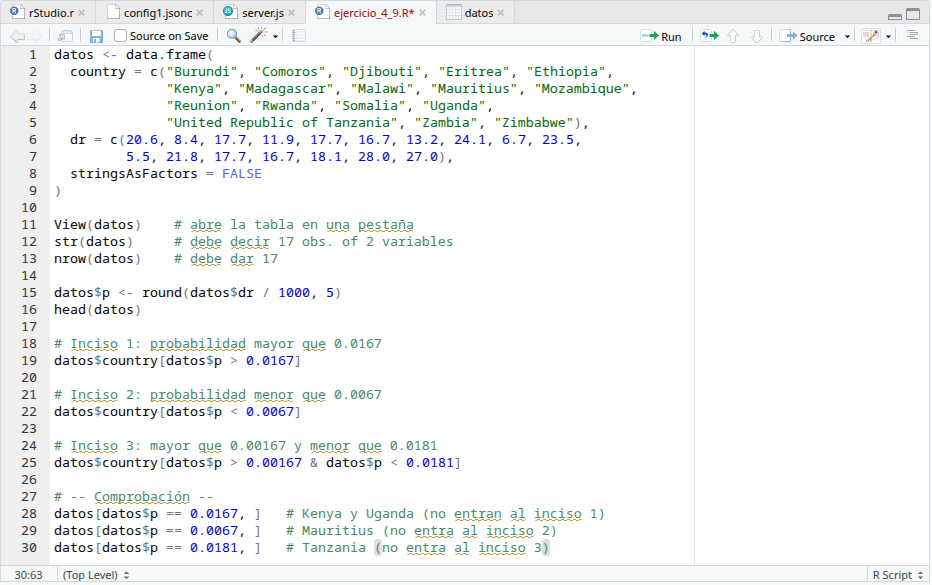
\includegraphics[width=0.82\textwidth]{img/1.png}
\caption{Probabilidad de mortalidad en África Oriental: conversión de tasas a probabilidades y filtrado de países por umbrales}
\end{figure}
 
\subsubsection*{Resultados}
\begin{itemize}
  \item \textbf{Inciso 1} ($p > 0.0167$, es decir, $\mathrm{dr} > 16.7$): Burundi, Djibouti, Ethiopia, Malawi, Mozambique, Rwanda, Somalia, United Republic of Tanzania, Zambia y Zimbabwe. Kenya y Uganda no se incluyen porque su tasa es exactamente $16.7$ y la desigualdad es estricta.
  \item \textbf{Inciso 2} ($p < 0.0067$, es decir, $\mathrm{dr} < 6.7$): únicamente Reunion ($5.5$). Mauritius tiene exactamente $6.7$, por lo que queda excluida.
  \item \textbf{Inciso 3} ($0.00167 < p < 0.0181$): Comoros, Djibouti, Eritrea, Ethiopia, Kenya, Madagascar, Mauritius, Reunion, Somalia y Uganda. La cota inferior no elimina ningún país, y United Republic of Tanzania queda excluida porque su tasa es exactamente $18.1$.
\end{itemize}

\begin{figure}[H]
\centering
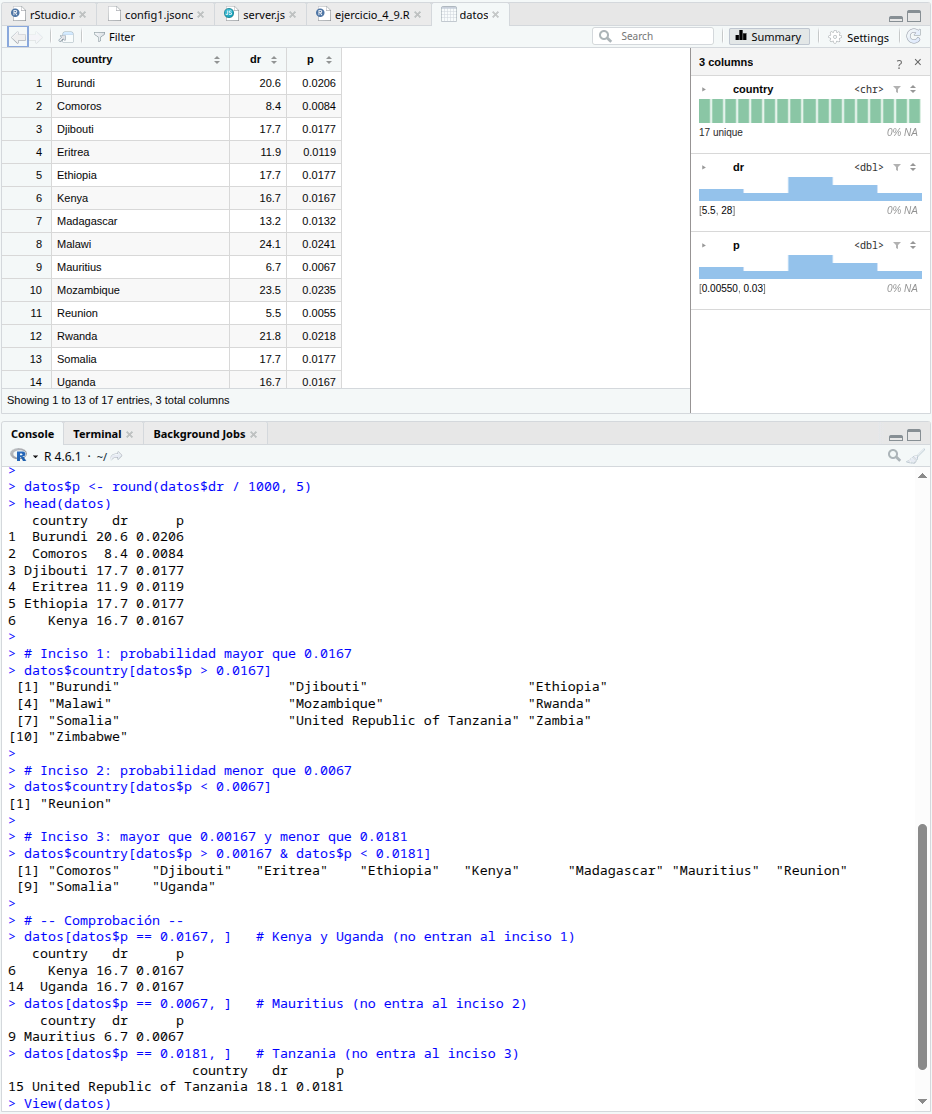
\includegraphics[width=0.92\textwidth]{img/2.png}
\caption{Ejecución del script}
\end{figure}
 
\textit{Observación:} si la cota inferior del inciso 3 fuera $0.0167$ en lugar de $0.00167$, el resultado serían solo Djibouti, Ethiopia y Somalia.
 
%==========================================================
\subsection{Ejercicio 4.21: tuberculosis y prueba diagnóstica}
 
\subsubsection*{Enunciado}
Se estudia una población en la que el $0.2\%$ de los individuos padece tuberculosis. Se aplica una prueba diagnóstica: de quienes tienen la enfermedad, el $98\%$ da positivo, y de quienes no la tienen, el $85\%$ da negativo. Se elige un individuo al azar y se le aplica la prueba. Sean $E$ el evento <<la persona tiene tuberculosis>> y $F$ el evento <<la prueba resulta positiva>>. Se pide:
\begin{itemize}
  \item Construir un diagrama de árbol con las probabilidades en cada rama.
  \item Calcular $P(E \cap F)$.
  \item Calcular $P(F)$.
  \item Calcular $P(E \mid F)$.
\end{itemize}
 
\subsubsection*{Datos}
\begin{itemize}
  \item Prevalencia: $P(E) = 0.002$, de donde $P(E^c) = 0.998$.
  \item Sensibilidad: $P(F \mid E) = 0.98$, de donde $P(F^c \mid E) = 0.02$.
  \item Especificidad: $P(F^c \mid E^c) = 0.85$, de donde $P(F \mid E^c) = 0.15$.
\end{itemize}
 
\subsubsection*{Desarrollo}
 
\paragraph{1. Diagrama de árbol.}
\begin{center}
  \begin{tikzpicture}[every node/.style={font=\small}]
    \node (r) at (0,0) {Persona};
    \node (e) at (3.2,1.7) {$E$};
    \node (n) at (3.2,-1.7) {$E^c$};
    \node[anchor=west] (ef) at (6.2,2.5) {$E \cap F$: $0.00196$};
    \node[anchor=west] (en) at (6.2,0.9) {$E \cap F^c$: $0.00004$};
    \node[anchor=west] (nf) at (6.2,-0.9) {$E^c \cap F$: $0.1497$};
    \node[anchor=west] (nn) at (6.2,-2.5) {$E^c \cap F^c$: $0.8483$};
    \draw[-latex] (r) -- node[above, sloped] {$0.002$} (e);
    \draw[-latex] (r) -- node[below, sloped] {$0.998$} (n);
    \draw[-latex] (e) -- node[above, sloped] {$0.98$} (ef.west);
    \draw[-latex] (e) -- node[below, sloped] {$0.02$} (en.west);
    \draw[-latex] (n) -- node[above, sloped] {$0.15$} (nf.west);
    \draw[-latex] (n) -- node[below, sloped] {$0.85$} (nn.west);
  \end{tikzpicture}
 
  \small\textit{Diagrama de árbol del Ejercicio 4.21 ($E$: con tuberculosis; $F$: prueba positiva).}
\end{center}
 
\paragraph{2. Probabilidad de tener la enfermedad y dar positivo.} Por la regla de la multiplicación:
\[
P(E \cap F) = P(E)\,P(F \mid E) = 0.002 \times 0.98 = 0.00196.
\]
 
\paragraph{3. Probabilidad de que la prueba sea positiva.} Por la ley de la probabilidad total:
\[
\begin{aligned}
P(F) &= P(E \cap F) + P(E^c \cap F) \\
     &= 0.00196 + 0.998 \times 0.15 \\
     &= 0.00196 + 0.1497 = 0.15166.
\end{aligned}
\]
 
\paragraph{4. Probabilidad de tener la enfermedad dado que la prueba es positiva.} Por el teorema de Bayes:
\[
P(E \mid F) = \frac{P(E \cap F)}{P(F)} = \frac{0.00196}{0.15166} \approx 0.0129.
\]
 
\subsubsection*{Cálculo en R}
\begin{lstlisting}[style=rstyle]
pE     <- 0.002   # prevalencia
pF_E   <- 0.98    # sensibilidad
pF_nE  <- 0.15    # 1 - especificidad
 
pEF    <- pE * pF_E                  # P(E y F)
pF     <- pEF + (1 - pE) * pF_nE     # P(F)
pE_F   <- pEF / pF                   # P(E | F)
 
round(c(P_E_y_F = pEF, P_F = pF, P_E_dado_F = pE_F), 5)
\end{lstlisting}
 
\subsubsection*{Resultados}
\begin{itemize}
  \item $P(E \cap F) = 0.00196$
  \item $P(F) = 0.15166$
  \item $P(E \mid F) \approx 0.0129$ (aproximadamente $1.3\%$)
\end{itemize}
 
\subsubsection*{Interpretación}
Aunque la prueba detecta al $98\%$ de los enfermos, solo cerca del $1.3\%$ de quienes dan positivo tienen realmente tuberculosis. Esto ocurre porque la enfermedad es muy poco frecuente ($0.2\%$) y el $15\%$ de los sanos da un falso positivo, de modo que los falsos positivos superan ampliamente a los verdaderos positivos. Es un ejemplo del efecto de la tasa base: un resultado positivo no equivale a un diagnóstico confirmado y requiere pruebas complementarias.

\end{document}